\subsection{Original}
\label{sec:310}

\todorev{Last revised and changed on Sat, June 30 at 15:24 by pfac}

The original \polu program was implemented using structures as \textit{Arrays-Of-Pointers} (AOP). While this allows for an easier development and better code readability, the deep levels of dereferencing imply an increased number of memory accesses, which aggravate the effects of any memory bottlenecks.

In this original version, the \computeflux function (see \cref{alg:flux}) iterates over each edge, and loads the pollution levels and velocity vectors of the cells it connects.
% For edges in the border of the mesh, a convention is followed, indicating that the non existing cell is always the right one (cells are refered to as left and right cells of a given edge). When the right cell does not exist, the \dirichlet condition is used as the value for that border.
A convention is followed (see \cref{fig:edge}), indicating that an edge always has a cell on its ``left'', and that the normal of the edge always points to its ``right'' cell. For the edges in the border of the mesh, the ``right'' cell does not exist. In this case, the \dirichlet condition is used as a the polution value in that hypothetical cell.

\begin{figure}
	\centering
	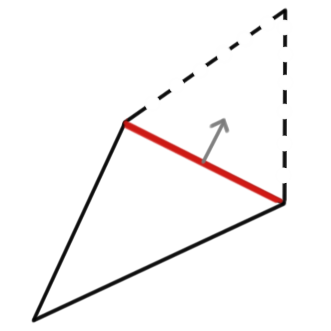
\includegraphics[width=.5\columnwidth]{images/edge-normal.png}
	\caption[An edge]{An edge. Every cell has at least one adjacent ``left'' cell. Border edges do not have a ``right'' cell. Edge normals always point to the ``right''.}
	\label{fig:edge}
\end{figure}

The value for the velocity in the edge is computed based on the velocity vectors of both adjacent cells and the normal of the edge.
The edges in the border assume for the hypothetical ``right'' cell a velocity equal to the ``left'' cell, which results in null flux.
Despite not being a vector, this computed velocity gives information about the direction of the flux:
a positive value represents the pollution flow from left to right; the inverse happens with a negative velocity.

This function also returns the elapsed time, which is computed with the maximum absolute value of the computed edge velocities, and is used at the end of the iteration to keep track of the total elapsed time.

\begin{figure}[!htp]
	\begin{alg}
		\ForAll {$edge \in Edges$}
			\State $l     \gets left\_cells_{edge}$
			\State $r     \gets rigth\_cells_{edge}$
			\State $u_{l} \gets pollution_{l}$
			\If {$\exists Cells_{r}$}
				\State $u_{r} \gets pollution_{r}$
			\Else
				\State $u_{r} \gets \dirichlet$ 
			\EndIf
			\State $v_{edge} \gets \dfrac{\vec{v}_{l} + \vec{v}_{r}}{2} \cdot \vec{n}_{edge}$
			\State $v_{max} \gets \mathrm{max}(v_{max}, v_{edge})$
			\State $flux_{edge} += u_{l} \cdot [v_{edge}]^{+} + u_{r} \cdot [v_{edge}]^{-}$
		\EndFor
		\State $\Delta t \gets |v_{max}|^{-1}$
		\State \Return $\Delta t$
	\end{alg}

	\caption{Pseudocode for the original \computeflux function.}
	\label{alg:flux}
\end{figure}

The original \update function also iterates over each edge.
The contribution of each edge to the cells final value is computed as the product between the elapsed time, the computed flux and the ratio between the edge's length and the cell's area.
This is illustrated in \cref{alg:update}.

\begin{figure}[!htp]
	\begin{alg}
		\ForAll {$edge \in Edges$}
			\State $\Delta{u} \gets \Delta{t} \cdot flux_{edge} \cdot L_{edge}$
			\State $l \gets left\_cells_{edge}$
			\State $r \gets right\_cells_{edge}$
			\State $pollution_{l} -= \frac{\Delta{u}}{A_{l}}$
			\If {$\exists Cells_{r}$}
				\State $pollution_{r} \gets \frac{\Delta{u}}{A_{r}}$
			\EndIf
		\EndFor
	\end{alg}

	\caption{Pseudocode for the original \update function.}
	\label{alg:update}
\end{figure}

In this original implementation, there is also the possibility to output the current state of the mesh after every $X$ iterations, where $X$ is a parameter provided in the configuration file loaded at runtime.
This feature allows the output to contain not only the final state of the system but all the intermediary states, allowing  an animation to be shown using \texttt{gmsh}.

\subsubsection{Simplifications}
% \todo[inline]{Animation and velocity calculation are out}

Two important simplifications were initially performed in the original version, before any other adaptation or rewrite of the code.

The first simplification meant removing the output operation at the end of each main loop iteration, thus removing the animation feature. While this feature is interesting to analyze how the system evolved, input/output operations are very slow when compared to computation operations. Since the main goal of this document is to study ways to improve the performance of the \polu application, this feature may be discarded.

The second major simplification focus on the \computeflux function. Since the every cell's velocity vector remains constant throughout the entire program's execution, the same values will be computed for the velocity in each edge and for the elapsed time. While this computation is important in a more dynamic application where velocity vectors are also updated, such is not the case for this algorithm. Therefore, it is possible to remove these two computational steps from the core function to the preprocessing stage, thus globally improving the program's performance.
